\chapter{Methodology}

% \section{Apparatus}

% \section{Procedure}

% \section{Measurements}

% \section{Participants}

\section{Android UI Data}
\subsection{Data tree structure}


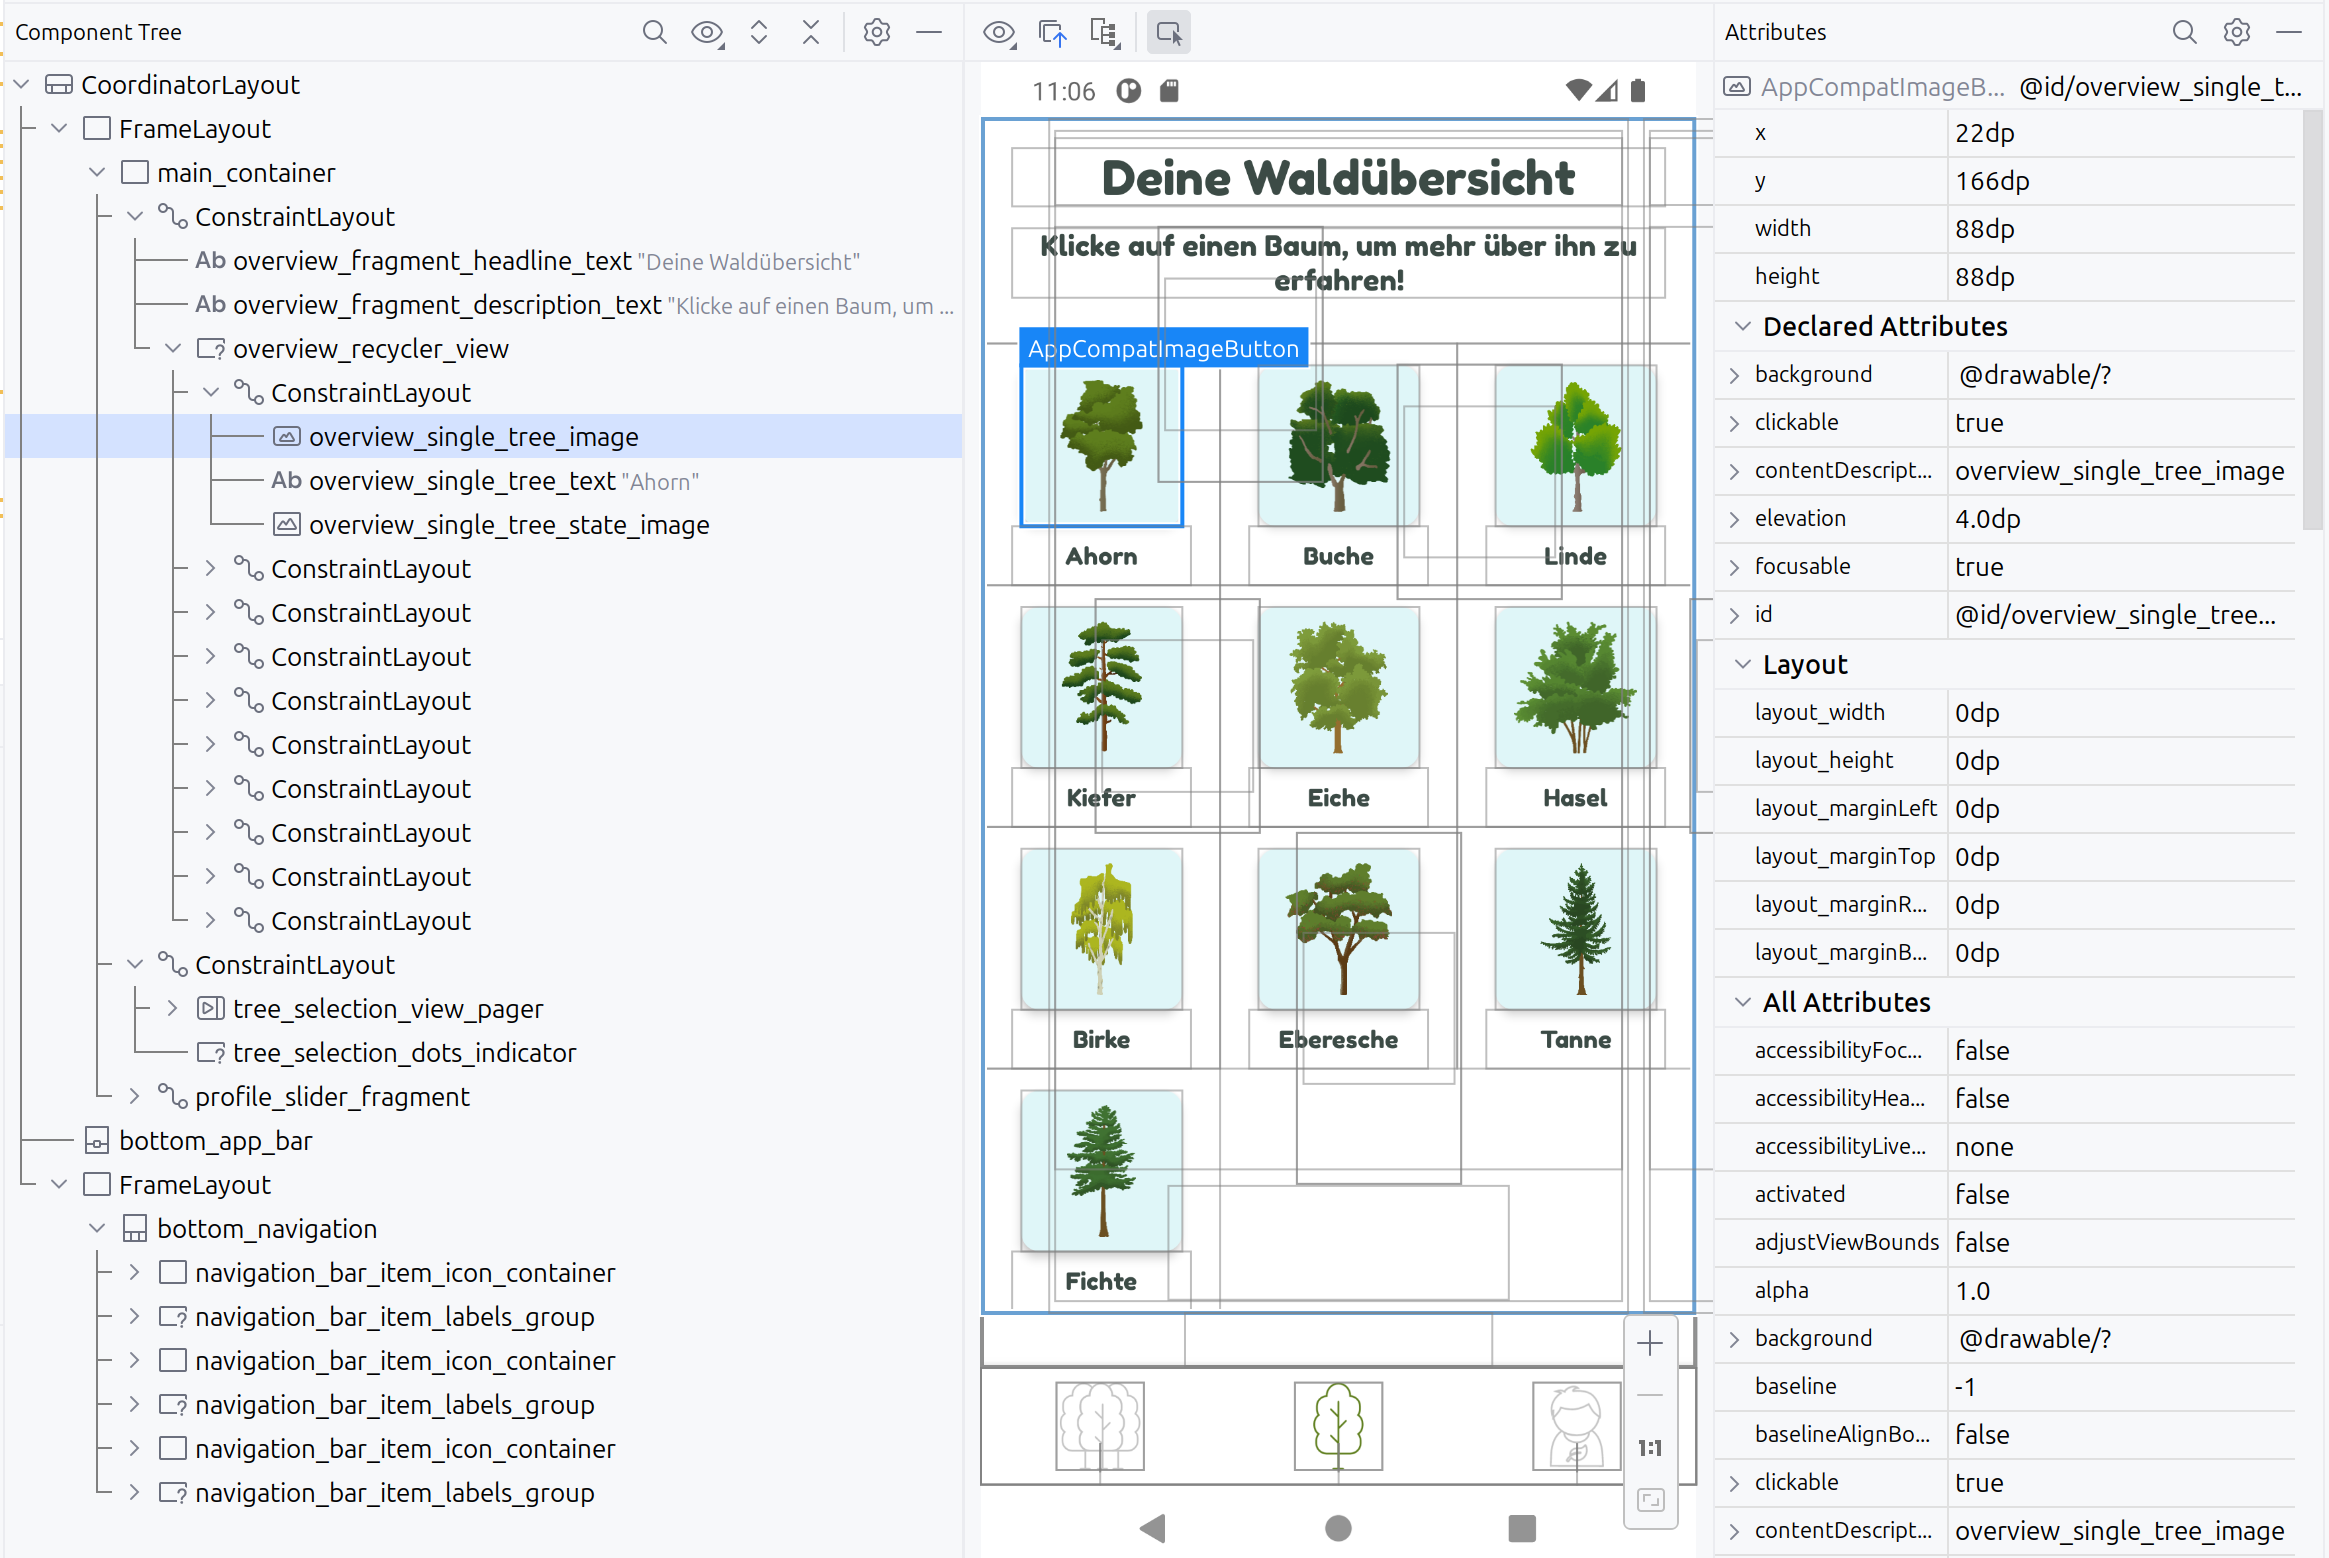
\includegraphics[width=\textwidth]{graphics/android_layout_inspector}
https://developer.android.com/studio/debug/layout-inspector

\subsection{Retrieval of UI data via Android Accessibility Service}

Semantics tree:
https://developer.android.com/jetpack/compose/semantics
https://android.googlesource.com/platform/frameworks/testing/+/jb-dev/uiautomator/library/src/com/android/uiautomator/core/AccessibilityNodeInfoDumper.java

\autoref{lst:ListingANDlstlisting,android_accessibility_node} zeigen, wie man Programmlistings einbindet.
https://github.com/mimuc/app-ins-gruene

\lstinputlisting[language=XML,label=android_accessibility_node,caption={Android Accessibility Node in XML.},float]{code/android_accessibility_node.xml}

\section{Machine Learning}
\subsection{Preprocessing}
\subsubsection{Normalization, Feature selection}

Such as Filtering privacy invasive details

Parameterizing the vectorization process
             a) Vector length
             b) Weighting of features
             c) Manipulating individual parameters of model
             
\subsection{Supervised vs Unsupervised vs Semisupervised}
\subsection{Under and Overfitting}
\subsection{Evaluation Metrics}
\subsection{Neuronal Nets}
Activation Functions
Cost function
Gradient
- Regression: Continous Values
- Classification: Multiple class
- One Class


Tensors
%https://stackoverflow.com/a/48599383/5164462

LSTM 4 dimensional
% https://stackoverflow.com/questions/54743549/is-it-possible-to-making-lstm-model-with-4-dimension-shape-of-data

Embedding before LSTM
% https://stackoverflow.com/questions/47217151/keras-lstm-with-embedding-layer-before-lstm-layer
% https://stackoverflow.com/questions/52627739/how-to-merge-numerical-and-embedding-sequential-models-to-treat-categories-in-rn/52629902#comment136040845_52629902

TimeDistributedLayer
% https://stackoverflow.com/a/61588937/5164462
% https://stackoverflow.com/questions/53107126/what-are-the-uses-of-timedistributed-wrapper-for-lstm-or-any-other-layers
\subsubsection{Deep Neuronal Nets}

\subsubsection{Convolutional Neuronal Nets}
\subsubsection{Recurrent Neuronal Networks and LSTMs / GRU}

\subsection{Layers}

- Embedding layer
    Dimension near the actual average length of features
- Dense Layer

Positive Integer to Dense Vectors of fixed size

\subsubsection{Autoencoders}
